\section{ Hauptteil }

\begin{frame}[plain]
    \centering
    \Large
    \textbf{Herleitung Selbstkonsistenzgleichung}
    \vspace{1cm}
    \begin{itemize}
        \item Ziel: Bestimmung von Energielücke $\Delta$ der supraleitender Phase
        \item Verwende dazu Mean-Field-Näherung und dessen Selbstkonsistenzgleichung
    \end{itemize}
\end{frame}


\begin{frame}
    \frametitle{Das Modell}
    \begin{itemize}
        \item Hamiltonian
        \begin{align*}
            \oH = \oH_{\text{TB}} + \oH_{\mu} + \oHWW
        \end{align*}
        \begin{align*}
            \oH_{\text{TB}} &= -t \sum_{\vec{R}, \vdelta, \sigma} \oad{\vec{R}, \sigma} \ob{\vec{R}+\vdelta, \sigma} + \hc &
            \oH_\mu &= - \mu \sum_{\vec{R}, \sigma} \sum_C \op{C}^{\dagg}_{\vec{R}, \sigma} \op{C}^{\pdagg}_{\vec{R}, \sigma} \\
            \oHWW &=  - \frac{U}{N} \sump{\vk, \vk'} \sum_\oC  \ocdu \ocdd \ocndd \ocndu 
        \end{align*}
        \item Schreibweise $\sum_{\vk}' = \sum_{\vk} \Theta(\hbar \omega_D - \abs{\epsilon_\vk - E_F})$
        \begin{itemize}
            \item[$\rightarrow$] Setze $E_F = 0$ damit das chemische Potential $\mu$ eine Verschiebung von $E_F$ beschreibt
        \end{itemize}
        \item $\sum_\oC  = $ Summe über Operatoren beider Untergitter
    \end{itemize}
\end{frame}

\begin{frame}
    \frametitle{Fourier-Trafo}
    \begin{itemize}
        \item Fourier-Trafo der Operatoren
        \begin{align*}
            \oc{\vec{R}} &= \frac{1}{\sqrt{N}} \sum_{\vk} \oc{\vk} e^{\im \vk \cdot \vec{R}}  & \ocd{\vec{R}} &= \frac{1}{\sqrt{N}} \sum_{\vk} \ocd{\vk} e^{-\im \vk \cdot \vec{R}}
        \end{align*}
        \item Damit lauten $\oH_\text{TB}$ und $\oH_\mu$ im Impulsraum
        \begin{align*}
            \oHTB &= \sum_{\vk, \sigma} f(\vk) \oakd \obk + \hc & \oH_\mu = - \mu \sum_{\vk, \sigma} \sum_\oC \ocd{\vk, \sigma} \oc{\vk, \sigma} 
        \end{align*}
        \item Es gilt $f(\vk) = -t \sum_{\vdelta} e^{\im \vk \cdot \vdelta} = -t \left(e^{(-\im k_x a)} + 2 \, e^{(\im k_x \frac{a}{2})} \cos\left(\frac{k_y a \sqrt{3}}{2}\right)\right)$

    \end{itemize}
\end{frame}

\begin{frame}
    \frametitle{Mean-Field-Näherung (1)}
    \begin{itemize}
        \item Gesamthamiltonian
        \begin{align*}
            \oH = \sum_{\vk, \sigma} \left(f(\vk) \oakd \obk + \hc - \mu \sum_\oC \ocd{\vk, \sigma} \oc{\vk, \sigma}\right) - \frac{U}{N} \sump{\vk, \vk'} \sum_\oC  \ocdu \ocdd \ocndd \ocndu
        \end{align*}
        \item Probleme der Diagonalisierung durch Wechselwirkungsterm
    \end{itemize}     
    \begin{minipage}[t]{0.5\textwidth}
        \begin{itemize}
            \item Mean-Field-Näherung reduziert auf ein Ein-Teilchen-Problem 
            \item Näherung gerechtfertigt, da bei Cooper-Paar-Kondensatbildung makroskopische Teilchenanzahl beteiligt $\rightarrow$ Fluktuationen vernachlässigbar
        \end{itemize}
    \end{minipage}
    \begin{minipage}[t]{0.49\textwidth}
        \begin{figure}[b]
            \centering
            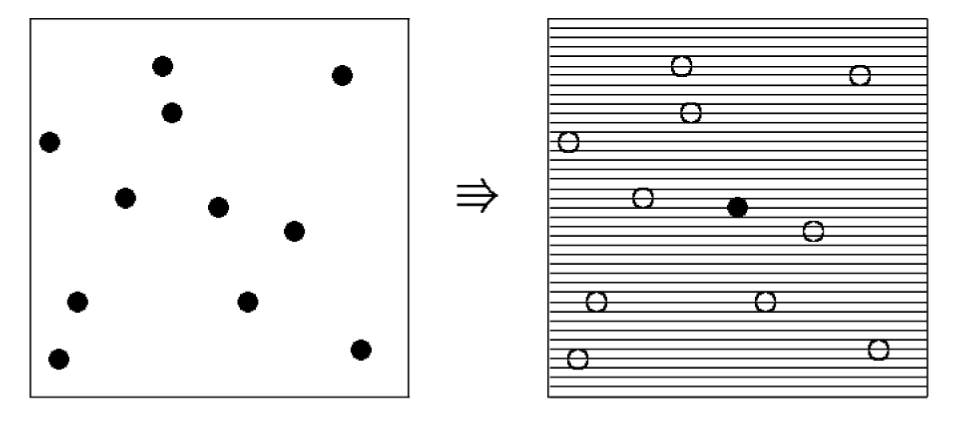
\includegraphics[width=\textwidth]{images/MF.png}
            \caption{Mean-Field-Näherung~\cite{bruus_manybody_2004}.}
            % \label{<label>}
        \end{figure}
    \end{minipage}
\end{frame}

\begin{frame}
    \frametitle{Mean-Field-Näherung (2)}
    \begin{itemize}
        \item Wick-Theorem
        \begin{align*}
            \ocdu \ocdd \ocndd \ocndu &= \, \only<1>{:\ocdu \ocdd \ocndd \ocndu:}\uncover<2->{\RedCancel{:\ocdu \ocdd \ocndd \ocndu:}}\\
            &\only<1-2>{\begin{aligned}
                &+ \expval{\ocdu \ocdd} \only<1>{:}\ocndd \ocndu\only<1>{:} + \expval{\ocndd \ocndu} \only<1>{:}\ocdu \ocdd\only<1>{:}\\
                &- \expval{\ocdu \ocndd} \only<1>{:}\ocdd \ocndu\only<1>{:} - \expval{\ocdd \ocndu} \only<1>{:}\ocdu \ocndd\only<1>{:}\\
                &+ \expval{\ocdu \ocndu} \only<1>{:}\ocdd \ocndd\only<1>{:} + \expval{\ocdd \ocndd} \only<1>{:}\ocdu \ocndu\only<1>{:}
            \end{aligned}}\uncover<3->{\left.\begin{aligned}
                &+ \expval{\ocdu \ocdd} \only<1>{:}\ocndd \ocndu\only<1>{:} + \expval{\ocndd \ocndu} \only<1>{:}\ocdu \ocdd\only<1>{:}\\
                &- \only<4>\RedCancel{\expval{\ocdu \ocndd} \only<1>{:}\ocdd \ocndu\only<1>{:} - \expval{\ocdd \ocndu} \only<1>{:}\ocdu \ocndd\only<1>{:}}\\
                &+ \expval{\ocdu \ocndu} \only<1>{:}\ocdd \ocndd\only<1>{:} + \expval{\ocdd \ocndd} \only<1>{:}\ocdu \ocndu\only<1>{:}
            \end{aligned}\right\}\begin{aligned}
                &\text{anomale Erwartungswerte}\\
                &\text{Fock-Term}\\
                &\text{Hartree-Term}
            \end{aligned}}\\
            &+ \only<1>{\text{const.}}\uncover<2->{\RedCancel{\text{const.}}}
        \end{align*}
    \item \uncover<2->{Mean-Field-Näherung: vernachlässige normalgeordneten quartischen Term}
    \item \uncover<2->{Nutze $: \op{c}\op{c}: = \op{c}\op{c} - \expval{\op{c} \op{c}} = \op{c}\op{c} - \text{const.}$ und vernachlässige Konstante}
    \item \uncover<4-> {Fock-Term verletzt Spinerhaltung $\rightarrow$ fällt weg}
    \end{itemize}
\end{frame}

\begin{frame}
    \frametitle{Mean-Fiel-Näherung -- Hartree-Term}
    \begin{itemize}
        \item Hartree-Term 
        \begin{align*}
            \expval{\ocdu \ocndu} \ocdd \ocndd + \expval{\ocdd \ocndd} \ocdu \ocndu
        \end{align*}
        \begin{itemize}
            \pause
            \item[$\rightarrow$] Impulserhaltung erzwingt $\vk = \vk'$ 
        \end{itemize}
        \pause
        \item eingesetzt in Wechselwirkungsterm 
        \begin{align*}
            \oH_\text{Hartree} &= -\frac{U}{N} \sum_\oC \sump{\vk} \left[\expval{\ocd{\vk, \up} \oc{\vk, \up}} \ocd{-\vk, \down} \ocndd + \expval{\ocd{-\vk, \down} \ocndd} \ocd{\vk, \up} \ocndu\right]
        \end{align*}
        \begin{itemize}
            \item[$\rightarrow$] skaliert nicht mit $N$, bleibt konstant bei $N \rightarrow \infty$
            \item[$\rightarrow$] andere Terme skalieren linear mit $N$ $\implies$ Hartree-Term im Limes $N \rightarrow \infty$ vernachlässigbar
        \end{itemize}
    \end{itemize}
\end{frame}

\begin{frame}
    \frametitle{Mean-Field-Näherung -- Cooper-Kanal}
    \begin{itemize}
        \item effektive Wechselwirkung damit nur Cooper-Kanal
        \begin{align*}
            \oHWWeff &= -\frac{U}{N} \sum_\oC \sump{\vk, \vk'}\left[\ocd{\vk, \up} \ocd{-\vk, \down} \expval{\oc{-\vk', \down} \oc{\vk', \up}} + \ocndd \ocndu \expval{\ocdu \ocdd}\right]
        \end{align*}
        \pause
        \item Definition Ordnungsparameter
        \begin{align*}
            \Delta_\oC &= \frac{U}{N} \sump{\vec{k}'} \expval{\oc{-\vk, \down} \ocndu} &\Delta_{\oC}^{*} &= \frac{U}{N} \sump{\vec{k}'} \expval{\ocdup \ocddown}
        \end{align*}
        \pause
        \begin{itemize}
            \item[$\rightarrow$] bei Supraleitung makroskopische Anzahl an Cooper-Paaren $\implies$ anomale Erwartungswerte nicht null 
            \item[$\rightarrow$] Bienenwabengitter hat Untergitter-Symmetrie $\implies$ $\Delta_\oA = \Delta_\oB$
            \item[$\rightarrow$] $\Delta$ kann wegen Eichsymmetrie des Systems reell gewählt werden
        \end{itemize}
        \pause
        \item damit effektive Wechselwirkung
        \begin{align*}
            \oHWWeff &= - \Delta \left(\sum_\oC \sump{\vk} \ocdup \ocddown + \hc\right)
        \end{align*}
    \end{itemize}
\end{frame}

% \begin{frame}
%     \frametitle{Mean-Field-Näherung (3)}
%     \begin{itemize}
%         \item wegen Impulserhaltung fällt Hartree-Term nur für $\vk = \vk'$ nicht weg und ergibt 
%         \begin{align*}
%             \oH_\text{Hartree} &= -\frac{U}{N} \sum_\oC \sump{\vk} \left[\expval{\ocd{\vk, \up} \oc{\vk, \up}} \ocd{-\vk, \down} \ocndd + \expval{\ocd{-\vk, \down} \ocndd} \ocd{\vk, \up} \ocndu\right]
%         \end{align*}
%         \begin{itemize}
%             \item[$\rightarrow$] skaliert nicht mit $N$ und ist im Limes $N \rightarrow \infty$ vernachlässigbar
%         \end{itemize}
%         \item Wechselwirkungsterm ist damit nur 
%         \begin{align*}
%             \oHWWeff &= - \sum_\oC \Delta_\oC \sump{\vk} \ocdup \ocddown + \hc
%         \end{align*}
%         \item Ordnungsparameter 
%         \begin{align*}
%             \Delta_\oC &= \frac{U}{N} \sump{\vec{k'}} \expval{\oc{-\vk, \down} \ocndu} & & \text{und} & \Delta_{\oC}^{*} &= \frac{U}{N} \sump{\vec{k'}} \expval{\ocdup, \ocddown}
%         \end{align*}
%     \end{itemize}
% \end{frame}

\begin{frame}
    \frametitle{Matrixschreibweise (1)}
    \begin{itemize}
        \item Gesamthamiltonian 
        \begin{align*}
            \oHeff &= \sum_{\vk, \sigma} \left[\left(f(\vk) \oakd \obk +\hc\right) - \mu \left( \oakd \oak + \obkd \obk \right) \right]  \\
            &- \Delta \sump{\vk} \left(\oadup \oaddown + \obdup \obddown + \hc \right) 
        \end{align*}
        \item Nambu-Spinore 
        \begin{align*}
            \vopsi &= \begin{pmatrix} \oadup \\  \obdup \\ \oadown \\ \obdown \end{pmatrix} & \vopsid = \begin{pmatrix} \oaup \, , & \obup\, , & \oaddown\, , & \obddown\end{pmatrix}
        \end{align*}
    \end{itemize}
\end{frame}

\begin{frame}
    \frametitle{Matrixschreibweise (2)}
    \begin{itemize}
        \item Mit Nambu-Spinoren umgeschrieben ergibt sich 
        \begin{align*}
            \oHeff &= \sump{\vk} \vopsid \dul{h} \, \vopsi 
        \end{align*}
        \item Matrix $\dul{h}$
        \begin{align*}
            \dul{h} = \begin{pmatrix} \mu & -f^*(\vk) & \Delta & 0 \\ -f(\vk) & \mu & 0 & \Delta \\ \Delta & 0 & -\mu & f^*(\vk) \\ 0 & \Delta & f(\vk) & -\mu \end{pmatrix}
        \end{align*}
        % \begin{itemize}
        %     \item[$\rightarrow$] Diagonalisieurng
        % \end{itemize}
    \end{itemize}
\end{frame}

\begin{frame}
    \frametitle{Diagonalisierung }
    \begin{itemize}
        % \item Um Selbstkonsistenz von $\Delta$ auszunutzen müssen die anomalen Erwartungswerte bestimmt werden 
        % \begin{itemize}
        %     \item[$\rightarrow$] Hamiltonian muss diagonalisiert werden
        % \end{itemize}
        \item Mit passender unitärer Trafo $\dul{U}$ kann $\oHeff$ diagonalisiert werden 
        \begin{align*}
            \oHeff &= \sump{\vk} \vophid \dul{h}_\text{diag} \, \vophi & \text{mit} & & \vophi &= \dul{U}^\dagg \vopsi
        \end{align*}
        \item (thermodynamische) Erwartungswerte der Quasiteilchenoperatoren $\vophi$
        \begin{align*}
            % \expval{\ophid_{i} \ophi_{j}} = F(E_{i}) \delta_{ij} = \left(\frac{1}{e^{\beta E_i} + 1}\right)\delta_{ij}
            \expval{\vophi \cdot \vophid}_{ij} = \expval{\ophi_{i} \ophid_{j}} &= \expval{1 -\ophid_{j}  \ophi_{i}} = (1 - F(E_i))\delta_{ij}
        \end{align*}
        \item Inverse Trafo liefert Erwartungswerte der Teilchenoperatoren $\vopsi$
        \begin{align*}
            \expval{\symbf{\Psi}^{\pdagg}_i \symbf{\Psi}^{\dagg}_j} = \expval{\opsi \cdot \opsid}_{ij} = \expval{\dul{U} \ophi \cdot \vophid \dul{U}^\dagger}_{ij} = \left(\dul{U} \expval{\ophi \cdot \vophid} \dul{U}^\dagg\right)_{ij}
        \end{align*}
    \end{itemize}
\end{frame}

\begin{frame}
    \frametitle{Selbstkonsistenz -- allgemeiner Fall}
    \begin{itemize}
        \item Erinnerung Definition von $\Delta$
        \begin{align*}
            \Delta &= \frac{U}{N}\sump{\vk} \expval{\oadown \oaup}
        \end{align*}
        \begin{itemize}
            \item[$\rightarrow$] Setze $\expval{\oadown \oaup}$ ein
        \end{itemize}
        \item Diagonalisierung liefert die Selbskonsistenzgeleichung 
        \begin{align*}
            \Delta &= \frac{U}{4N} \sump{\vk} \left[\frac{\Delta}{E_+} \tanh\left(\frac{\beta E_+}{2}\right) + \frac{\Delta}{E_-} \tanh\left(\frac{\beta E_-}{2}\right)\right]
        \end{align*}
        \begin{itemize}
            \item[$\rightarrow$] Quasiteilchenenergien $E_\pm = \sqrt{(\epsilon_{\mp} - \mu)^2 + \Delta^2}$ mit Ein-Teilchen-Energien $\epsilon_\pm = \pm \abs{f(\vk)}$ 
        \end{itemize}
        \pause
        \item Alternative Schreibweise über Zustandsdichte $\rho(\epsilon) = \frac{1}{N} \sum_{\vk} \delta(\epsilon - \epsilon_\vk)$
        \begin{align*}
            \Delta = \frac{U}{2} \int_{\mu -\hbar \omega_D}^{\mu + \hbar \omega_D} d\epsilon \, \rho(\epsilon) \frac{\Delta}{\sqrt{(\epsilon - \mu)^2 + \Delta^2}} \tanh\left(\frac{\beta \sqrt{(\epsilon - \mu)^2 + \Delta^2}}{2}\right)
        \end{align*}
        % \begin{itemize}
        %     \item[$\rightarrow$] nun explizite Schreibweise des Cutoffs möglich
        % \end{itemize}
    \end{itemize}
\end{frame}

\begin{frame}
    \frametitle{Selbstkonsistenz -- Spezialfall halber Füllung}
    \begin{minipage}[t]{0.6\textwidth}
        \begin{itemize}
            \item Im Nächste-Nachbar-Tight-Binding-Modell ist das Bienenwabengitter bei $\mu = 0$ zur Hälfte gefüllt
            \item Für die Selbstkonsistenz ergibt sich 
            \begin{align*}
                \Delta = \frac{U}{2N} \sump{\vk} \frac{\Delta}{E_\vk} \tanh\left(\frac{\beta E_\vk}{2}\right)
            \end{align*}
            \item In Integralform
            \begin{align*}
                \Delta = \frac{U}{2} \int_{-\hbar \omega_D}^{\hbar \omega_D} d\epsilon \, \rho(\epsilon) \frac{\Delta}{\sqrt{\Delta^2 + \epsilon^2}} \tanh\left(\frac{\beta \sqrt{\Delta^2 + \epsilon^2}}{2}\right)
            \end{align*}
            \begin{itemize}
                \item[$\rightarrow$] Exakt das BCS Ergebnis für ein Band
            \end{itemize}
        \end{itemize}
    \end{minipage}
    \begin{minipage}[t]{0.39\textwidth}
        \begin{figure}
            \centering
            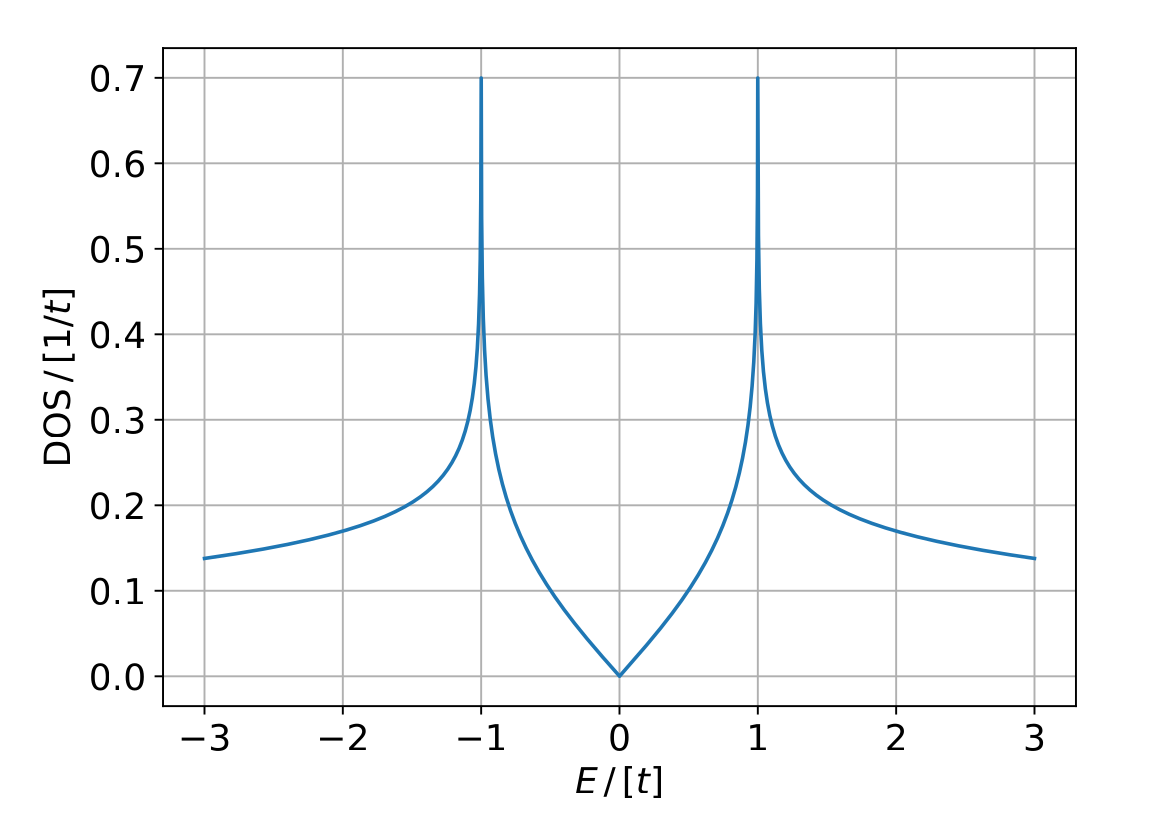
\includegraphics[width=\textwidth]{images/DOS.png}
            \caption{Zustandsdichte (DOS) Bienenwabengitter.}
            % \label{<label>}
        \end{figure}
    \end{minipage}
\end{frame}

\begin{frame}[plain]
    % \frametitle{Ergebnisse}
    \centering
    \Large
    \textbf{Ergebnisse}
\end{frame}